\documentclass[fleqn]{beamer}
\usetheme[english]{KIT}

\usepackage[utf8]{inputenc}
\usepackage[T1]{fontenc}
\usepackage{babel}
\usepackage{tikz,calc,ifthen}
\usepackage{mathtools}
\usepackage{amssymb}
\usepackage{amsmath}
\usepackage{MnSymbol}
\usepackage{stmaryrd}
\usepackage{bbold}
\usepackage[normalem]{ulem}
\usepackage{graphicx}
\usepackage{listings}
\usepackage{color}
\usepackage{colonequals}
\usepackage{mathpartir}

\definecolor{keywordcolor}{rgb}{0.7, 0.1, 0.1}   % red
\definecolor{commentcolor}{rgb}{0.4, 0.4, 0.4}   % grey
\definecolor{symbolcolor}{rgb}{0.0, 0.1, 0.6}    % blue
\definecolor{sortcolor}{rgb}{0.1, 0.5, 0.1}      % green
\def\lstlanguagefiles{lstlean.tex}
\lstset{language=lean}

\usetikzlibrary{positioning,calc,arrows,shapes}
\tikzset{
  every node/.style={transform shape},
  auto,
  block/.style={align=center,rectangle,draw,minimum height=20pt,minimum width=30pt},
  >=triangle 60,
  alt/.code args={<#1>#2#3}{%
      \alt<#1>{\pgfkeysalso{#2}}{\pgfkeysalso{#3}}
  },
  beameralert/.style={alt=<#1>{color=green!80!black}{}},
  mythick/.style={line width=1.4pt}
}

\newcommand*{\maxwidthofm}[2]{\maxof{\widthof{$#1$}}{\widthof{$#2$}}}
\newcommand<>*{\robustaltm}[2]{
  \alt#3
  {\mathmakebox[\maxwidthofm{#1}{#2}]{#1}\vphantom{#1#2}}
    {\mathmakebox[\maxwidthofm{#1}{#2}]{#2}\vphantom{#1#2}}
}

\newcommand<>*{\nodealert}[1]{\only#2{\draw[overlay,mythick,color=green!80!black] (#1.north west) rectangle (#1.south east)}}

\title{Static Uniqueness Analysis for the Lean 4 Theorem Prover}
\author{Marc Huisinga}
\subtitle{\insertauthor}
\institute[IPD]{Lehrstuhl Programmierparadigmen, IPD Snelting}
\date{08.05.2023}
\KITtitleimage{title.png}

\begin{document}

\begin{frame}
  \maketitle
\end{frame}

\begin{frame}{Compilation of Lean 4}
	\textbf{Lean 4:} Dependently typed theorem prover \& \underline{programming language}
	
	\vfill
	\setlength{\mathindent}{0pt}
	\begin{align*}
	\text{\textbf{Old:} Lean 4}\ &\underset{\text{C}}{\rightsquigarrow}\ \text{LCNF} \tag*{[Full type erasure]} \\
	&\underset{\text{C}}{\rightsquigarrow}\ \text{Pure IR} \\
	&\underset{\text{C}}{\rightsquigarrow}\ \text{\underline{Reference-counted} IR} \\
	&\underset{\text{C}}{\rightsquigarrow}\ \text{C}
	\end{align*}
	
	\vfill
	
	\begin{align*}
	\text{\textbf{WIP:} Lean 4}\ &\underset{\text{Lean}}{\rightsquigarrow}\ \text{LCNF} \tag*{[Type dependency erasure]} \\
	&\underset{\text{Lean}}{\rightsquigarrow}\ \text{\underline{Reference-counted} LCNF} \\ 
	&\underset{\text{Lean}}{\rightsquigarrow}\ \text{C \& LLVM} \tag*{[Full type erasure]}
	\end{align*}
\end{frame}

\begin{frame}{In-Place Updates (Counting Immutable Beans)}
	\textbf{Idea:} $\mathrm{RC}(v) = 1 \implies \text{safe ``in-place update'' of } v$
	
	\vfill
	
	\textbf{Destructive update:}\\ 
	$\mathrm{RC}(v) = 1\ \ \land\ \ v \text{ dead}\ \ \land\ \ \text{new memory allocated}$\\ 
	$\qquad\implies \text{reuse memory of } v$
	
	\vfill
	
	\textbf{In-place update of array:}\\
	$\mathrm{RC}(v) = 1\ \ \land\ \ v : \text{Array}\ \alpha \ \ \land\ \ f \in \{\text{set}, \text{push}, \text{pop}, \dots\}$\\
	$\qquad\implies v' = f(\dots, v, \dots) \text{ mutates } v$
\end{frame}

\begin{frame}{Motivation}
	\textbf{Central idea:} Referential uniqueness can be unintuitive \\
	$\qquad \implies$ Use static analysis to guarantee it
	
	\vfill
	
	\textbf{Bonus:} Statically guaranteed referential uniqueness enables optimizations, e.g.:
	\begin{itemize}
		\item No reference counting necessary
		\item More efficient update operations
		\item No aliasing!
	\end{itemize}

	\vfill
	
	\textbf{Approach:} Use a type theory to ensure referential uniqueness
\end{frame}

\begin{frame}{Substructural Type Theory}
	\underline{Substructural} type theories omit one of the following \underline{structural} rules:
	\begin{mathpar}
		$\inferrule[Exchange]{\Gamma_1, y : \tau_2, x : \tau_1, \Gamma_2 \vdash e : \tau}{\Gamma_1, x : \tau_1, y : \tau_2, \Gamma_2 \vdash e : \tau}$ \hspace{1.5em}
		$\inferrule[Weaken]{\Gamma \vdash e : \tau}{\Gamma, x : \tau' \vdash e : \tau}$ \hspace{1.5em}
		$\inferrule[Contract]{\Gamma, x : \tau', x : \tau' \vdash e : \tau}{\Gamma, x : \tau' \vdash e : \tau}$
	\end{mathpar}

	\vfill
	
	\textbf{Idea 1 (Girard, Wadler):} Omit \textsc{Weaken} + \textsc{Contract} and use $\Gamma$ to count variable uses in order to track resource usage and prevent aliasing
	
	\vfill
	
	\textbf{Idea 2 (Girard, Wadler):} Make substructurality an optional property of $\tau'$ for $x : \tau' \in \Gamma$ 
\end{frame}

\begin{frame}{(Invariably Unique) Linear Type Theory}
	$\tau'$, $\tau$ \underline{linear} types:
	\begin{align*}
		\Gamma, x : \tau' \vdash e : \tau \implies &x\ \text{is used exactly once} \\
		&\text{to create exactly one instance of}\ e
	\end{align*}
	
	\vfill
	
	\begin{mathpar}
		$\inferrule[Var]{ }{x : \tau \vdash x : \tau}$ \hspace{1.5em}
		$\inferrule[$\multimap$-Intro]{\Gamma, x : \tau_1 \vdash e : \tau_2}{\Gamma \vdash \lambda x : \tau_1.\ e : \tau_1 \multimap \tau_2}$ \hspace{1.5em}
		$\inferrule[$\multimap$-Elim]{\Gamma_1 \vdash e_1 : \tau_1 \multimap \tau_2 \\ \Gamma_2 \vdash e_2 : \tau_1}{\Gamma_1, \Gamma_2 \vdash e_1\ e_2 : \tau_2}$
	\end{mathpar}
\end{frame}

\begin{frame}{(Invariably Unique) Linear Type Theory}
	$!\tau'$, $!\tau$ \underline{nonlinear} types:
	\begin{align*}
		\Gamma, x :\ !\tau' \vdash e :\ !\tau \implies &x\ \text{is used arbitrarily often} \\
		&\text{to create arbitrarily many instances of}\ e
	\end{align*}

	\vfill
	
	\begin{mathpar}
		$\inferrule[Var]{ }{x : \tau \vdash x : \tau}$ \hspace{1.5em}
		$\inferrule[$\multimap$-Intro]{\Gamma, x : \tau_1 \vdash e : \tau_2}{\Gamma \vdash \lambda x : \tau_1.\ e : \tau_1 \multimap \tau_2}$ \hspace{1.5em}
		$\inferrule[$\multimap$-Elim]{\Gamma_1 \vdash e_1 : \tau_1 \multimap \tau_2 \\ \Gamma_2 \vdash e_2 : \tau_1}{\Gamma_1, \Gamma_2 \vdash e_1\ e_2 : \tau_2}$
	\end{mathpar}
	\begin{mathpar}
		$\inferrule[Weaken]{\Gamma \vdash e : \tau}{\Gamma, x :\ !\tau' \vdash e : \tau}$ \hspace{1.5em}
		$\inferrule[Contract]{\Gamma, x :\ !\tau', x :\ !\tau' \vdash e : \tau}{\Gamma, x :\ !\tau' \vdash e : \tau}$ 
	\end{mathpar} 
	\begin{mathpar}
		$\inferrule[!-$\multimap$-Intro]{!\Gamma, x : \tau_1 \vdash e : \tau_2}{!\Gamma \vdash \lambda x : \tau_1.\ e :\ !(\tau_1 \multimap \tau_2)}$ \hspace{1.5em}
		$\inferrule[!-$\multimap$-Elim]{\Gamma_1 \vdash e_1 :\ !(\tau_1 \multimap \tau_2) \\ \Gamma_2 \vdash e_2 : \tau_1}{\Gamma_1, \Gamma_2 \vdash e_1\ e_2 : \tau_2}$
	\end{mathpar}

	\vfill

	Invariable unique linear types are referentially unique!
\end{frame}

\begin{frame}{(Properly) Linear Type Theory}
	\textbf{Idea 1 (Girard, Wadler):} $x :\ !\tau'$ can be understood as having an unlimited quantity of $x$ 
	
	\vfill
	
	\textbf{Idea 2 (Girard, Wadler):} $x :\ !\tau' \implies x : \tau'$
	
	\vfill
	
	\begin{mathpar}
		$\inferrule[Dereliction]{\Gamma, x : \tau_1 \vdash e : \tau_2}{\Gamma, x :\ !\tau_1 \vdash e : \tau_2}$ \hspace{1.5em}
		$\inferrule[Promotion]{!\Gamma \vdash e : \tau}{!\Gamma \vdash e :\ !\tau}$ \hspace{1.5em}
		$\inferrule[Weaken]{\Gamma \vdash e : \tau}{\Gamma, x :\ !\tau' \vdash e : \tau}$ \hspace{1.5em}
		$\inferrule[Contract]{\Gamma, x :\ !\tau', x :\ !\tau' \vdash e : \tau}{\Gamma, x :\ !\tau' \vdash e : \tau}$
	\end{mathpar} 
	\begin{mathpar}
		$\inferrule[Var]{ }{x : \tau \vdash x : \tau}$ \hspace{1.5em}
		$\inferrule[$\multimap$-Intro]{\Gamma, x : \tau_1 \vdash e : \tau_2}{\Gamma \vdash \lambda x : \tau_1.\ e : \tau_1 \multimap \tau_2}$ \hspace{1.5em}
		$\inferrule[$\multimap$-Elim]{\Gamma_1 \vdash e_1 : \tau_1 \multimap \tau_2 \\ \Gamma_2 \vdash e_2 : \tau_1}{\Gamma_1, \Gamma_2 \vdash e_1\ e_2 : \tau_2}$
	\end{mathpar}

	\vfill
	
	\textbf{Problem:} $\Gamma, x : \tau' \vdash e : \tau$ does not guarantee referential uniqueness of $x$! \\
	\qquad(By \textsc{Dereliction})

\end{frame}

\begin{frame}{Uniqueness Type Theory}
	\textbf{Notation:} A substructural $\tau$ is written as $*\tau$
	
	\vfill
	
	\textbf{Idea 1 (Barendsen, Smetsers):} $x : *\tau'$ can be understood as $x$ being (referentially) unique
	
	\vfill
	
	\textbf{Idea 2 (Barendsen, Smetsers):} $x : *\tau' \implies x :\ !\tau'$
	
	\vfill
	
	\begin{mathpar}
		$\inferrule[Cast-Left]{\Gamma, x :\ !\tau' \vdash e : \tau}{\Gamma, x : *\tau' \vdash e : \tau}$ \hspace{1.5em}
		$\inferrule[Cast-Right]{\Gamma \vdash e : *\tau}{\Gamma \vdash e :\ !\tau}$
	\end{mathpar}

	\vfill
	
	... well-suited for our problem!
\end{frame}

\begin{frame}{Temporal Overview}
	\begin{center}
		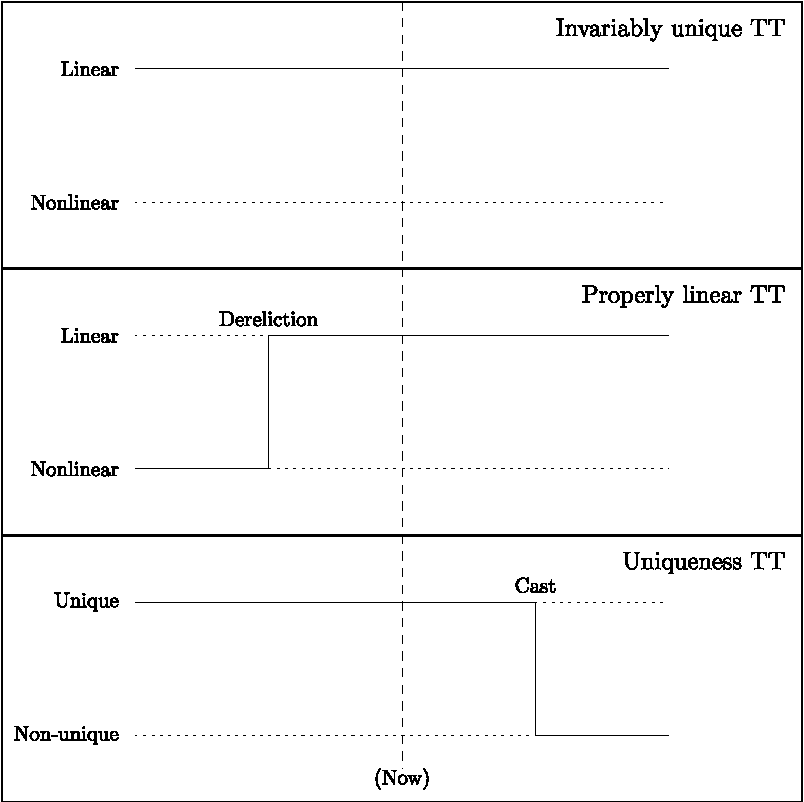
\includegraphics[height=0.95\textheight]{temporal_substructurality.pdf}
	\end{center}
\end{frame}

\begin{frame}{Nested Uniqueness 1}
	\textbf{Invariant ($I$):} Unique values cannot be stored within non-unique values.
	
	\vfill
	
	\textbf{Linear type theory:} Enforcing $I$ at construction is sufficient: \\
	\qquad To construct $!(\alpha \otimes \beta)$, we need $!\alpha$ and $!\beta$.
	
	\vfill
	
	\textbf{Uniqueness type theory:} $*(*\alpha \times *\beta)$ can be casted to $!(*\alpha \times *\beta)$ \\
	\qquad $\implies$ $I$ must be enforced after casting. \vspace{1em}
	
	Options:
	\begin{enumerate}
		\item Enforce $I$ at deconstruction: $!(*\alpha \times *\beta)$ cannot be deconstructed
		\item Enforce $I$ when casting: $!(*\alpha \times *\beta)$ is normalized to $!(!\alpha \times\ !\beta)$
	\end{enumerate}
	
\end{frame}

\begin{frame}{Nested Uniqueness 2}
	What about higher-order functions?
	
	\vfill
	
	\textbf{Problem:} $f : *(\alpha \to \beta)$ may contain a value $x : *\gamma$ in its closure. \\
	Cast to $f :\ !(\alpha \to \beta)$ $\implies$ $x$ can be duplicated by repeatedly calling $f$
	
	\vfill
	
	\textbf{Solutions:}
	\begin{enumerate}
		\item Make unique functions behave properly linear
		\item Make closure part of function type
		\item Argue \textsc{Cast} away using higher-ranked polymorphism
		\item \textsc{Cast} converts $f$ to a function that cannot make use of uniqueness
	\end{enumerate}
\end{frame}

\begin{frame}{Borrowing in Purely Functional Languages}
	\textbf{Problem:} Non-escaping parameters have to be returned explicitly to retain their uniqueness. \\
	
	\vfill
	
	\textbf{Example:} $\text{Array.get?} : *(\text{Array}\ !\alpha) \to\ !\text{Nat} \to\ !\alpha$ \\
	\begin{itemize}
		\item $\text{Array.get?} : *(\text{Array}\ !\alpha) \to\ !\text{Nat} \to\ *(*(\text{Array}\ !\alpha)\ \times\ !\alpha)$ $\implies$ ugly
		\item $\text{Array.get?} :\ !(\text{Array}\ !\alpha) \to\ !\text{Nat} \to\ !\alpha$ $\implies$ requires \textsc{Cast}
	\end{itemize}

	\vfill

	\textbf{Idea:} Non-escaping parameters $x :\ !\alpha$ do not consume arguments $x : *\alpha$. \\
	\qquad ($x$ does not escape in $f$ $\implies$ $x$ cannot be duplicated by $f$)
\end{frame}

\begin{frame}{Uniqueness for Lean 4: Basic Ideas}
	\textbf{Problem:} Combining dependent types with uniqueness types is hard, but types are nonetheless helpful information\vspace{0.5em}
	\setlength{\mathindent}{0pt}
	\setlength{\belowdisplayskip}{0pt}
	\setlength{\abovedisplayskip}{0pt}
	\begin{align*}
		\text{\textbf{Idea:} Lean 4}\ &\underset{\text{Lean}}{\rightsquigarrow}\ \text{LCNF} \tag*{[Type dependency erasure]} \\
		&\underset{\text{Lean}}{\rightsquigarrow}\ \text{\underline{Reference-counted} LCNF} \tag*{\textbf{[Uniqueness analysis]}}\\ 
		&\underset{\text{Lean}}{\rightsquigarrow}\ \text{C \& LLVM} \tag*{[Full type erasure]}
	\end{align*}

	\vfill

	\textbf{Problem:} What are the uniqueness attributes of fields of ADTs? \\
	\textbf{Idea:} An ADT field of type $*\alpha$ is unique if the ADT is unique.
	
	\vfill
	
	\textbf{Problem:} Type-based escape analyses escalate notational complexity. \\
	\textbf{Idea:} Design and implement an escape data-flow analysis.
\end{frame}

\begin{frame}{Uniqueness for Lean 4: Implementation}
	Prototype implementation of type checker using Lean 4 at \url{https://github.com/mhuisi/Uniq}
	
	\vfill 
	
	\begin{itemize}
		\item Targets a model of Lean 4's LCNF
		\item Implements the IR, the type system, an escape analysis, a borrow checker and the type checker
		\item \textasciitilde1kloc of Lean 4 code
	\end{itemize}
\end{frame}

\begin{frame}{Uniqueness for Lean 4: Limitations}
	Still missing:
	\begin{itemize}
		\item Uniqueness for higher-order functions
		\item Uniqueness attribute inference
		\item Uniqueness attribute polymorphism
		\item Full integration with Lean 4 compiler toolchain
		\item Proof of correctness
	\end{itemize}

	\vfill
	
	... But thesis outlines concrete ideas for future work on all of these!
\end{frame}

\begin{frame}{Closing}
	\begin{itemize}
		\item Is it possible to ensure referential uniqueness using a properly linear type theory and how would that compare to uniqueness type theory?
		\item Can uniqueness be integrated with quantitative type theory (combination of dependent and properly linear type theory)?
		\item What other approaches are there to implement borrowing?
		\item How to combine ADTs with borrowing?
		\item How to deal with ADT projections like $\text{fst} : *(*\alpha \times *\beta) \to *\alpha$?
		\item How to deal with types defined via FFI or erased types?
		\item How does our type theory compare with other substructural type theories for purely functional languages?
	\end{itemize}

	\vfill

	... Thanks for listening!
\end{frame}

\end{document}
